\chapter{Referencial Teórico}
    No decorrer da pesquisa elaborou-se um estudo a respeito das tecnologias com propostas como deste trabalho, métodos de desenvolvimento de software e tecnologias que melhor atendem às necessidades do projeto, as escolhas foram tomadas com a condição prévia de que poderiam ser aplicável a criação de aplicativos para smartphone.


\section{Pessoas como Sensores Voluntários}
    Para a compreensão da utilização de pessoas como sensores vê-se necessário o entendimento dos conceitos de User-generated content (UGC), World Wide Web 2.0 (WEB 2.0), Neogeografia, Inteligência Coletiva, e Volunteered Geographic Information (VGI), os quais serão apresentados a seguir. 

    UGC (User-Genereted Content – Conteúdo Gerado pelo Usuário) segundo \citeonline{santos_avaliacao_2016}, se refere a ação dos usuários compartilharem suas experiências e com isso produzir um grande volume de informações. Um dos mais populares exemplos é a Wikipédia, uma plataforma colaborativa que contém mais de 1.000,000 artigos em português e 6,292 usuários ativos, este número vem crescendo constantemente \cite{Wikipedia2018}.

    A WEB 2.0 representa uma maneira diferente de interagir com a internet, pois oferece maior autonomia para o usuário no sistema, na medida em que possibilita a criação de conteúdo e avaliação dos conteúdos consumidos. \citeonline [p.~2]{Primo2007} afirma que Web  2.0 é uma nova geração de serviços na rede, identificada por suas diversas formas de produção contributiva e partilhamento de informações online. Plataformas como Twitter e Youtube, com centenas de milhões de usuários, tem se adaptando para melhor atender seu público por meio da implementação de recursos que facilitam tanto a criação quanto à visualização de conteúdo. 

    O termo Neogeografia para \citeonline[p.~228]{machado_os_2014}, se trata de um fenômeno social que gira em torno do crescimento em massa dos mapas virtuais, e ao facilitamento de uso de tecnologias com ferramentas para posicionamento como o GPS.

   Para \citeonline[p.~28]{Levy2007}, inteligência coletiva é “uma inteligência distribuída por toda parte, incessantemente valorizada, coordenada em tempo real, que resulta em uma mobilização efetiva das competências”.

    De acordo com \apudonline[p.~10]{Goodchild2007}{miranda_uma_2010}, VGI é uma expressão usada para definir a informações geográficas que são produzidas através de usuários, que funde elementos da Web 2.0, Inteligência Coletiva e Neogeografia e que atinge as necessidades da indústria, do governo e comunidades de redes sociais. O conjunto de dados e as informações deles decorrentes são, através de plataformas de inteligência coletiva, avaliados, validados e consolidados pelos usuários, inclusive aqueles que geraram a informação.


\section{Engenharia de Software}
    Engenharia de software é um estudo que oferecem métodos para melhorar a produção e pode ser utilizada para projetar qualquer sistema, a definição dada por \citeonline[p. ~3]{ian_sommerville} diz que a engenharia de software é um apoio ao desenvolvimento de programa profissional, usando procedimento condizente aos critérios do sistema e auxiliam na evolução do programa, essas técnicas são aplicadas em documentações que se associam aos dados e apresentam as configurações necessárias para o funcionamento correto.
    
    As documentações são compostas por modelos de desenvolvimento, que define as etapas para construir o software; os requisitos, que especificam as funcionalidades que o  sistema deve executar; as regras de negócio, são restrições necessárias para o sistema; diagramas em UML que mostram interações e especificações em diagramas de fácil entendimento.


    \subsection{Modelo cascata}
        O modelo em cascata segue uma linha sequencial dividido em fases de desenvolvimento, como mostra as Figuras \ref{fig:cascata} e \ref{fig:flux}. É um modelo que exige uma analise inicial para definir as necessidades das funcionalidades do software. Em seguida, é necessário elaborar um projeto baseado nos requisitos que definirão a arquitetura geral, para que depois seja executada a implementação e o teste unitário, onde o desenvolvimento é realizado em unidades que são avaliadas para garantir que cada unidade atenda as especificações. A fase seguinte é integração e teste do sistema no qual as unidades desenvolvidas separadamente são integradas e testadas como um conjunto para e ser entregue ao cliente. Por fim vem a operação e manutenção que consiste em corrigir erros e melhorar e ampliar o programa \cite[p.~20]{ian_sommerville}.
    
        % Modelo cascata
        \begin{figure}[H]
        	\centering
        	\caption{Modelo cascata.}	
        	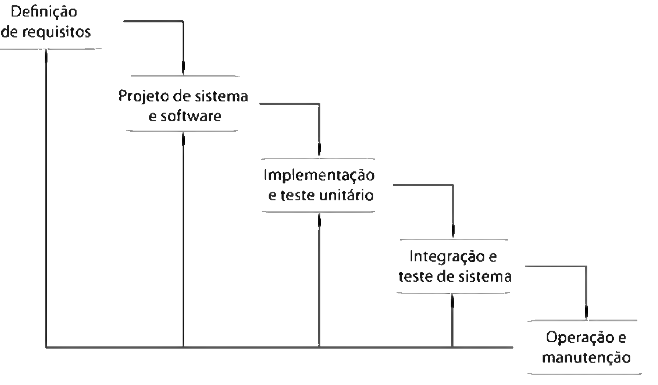
\includegraphics[width=\linewidth, frame]{Imagens/cascata}
        	\legend{Fonte: \cite[p.~20]{ian_sommerville}}
        	\label{fig:cascata}
        \end{figure}
        
        % Fluxograma
        \begin{figure}[H]
        	\centering
        	\caption{Fluxograma das fases de desenvolvimento.}	
        	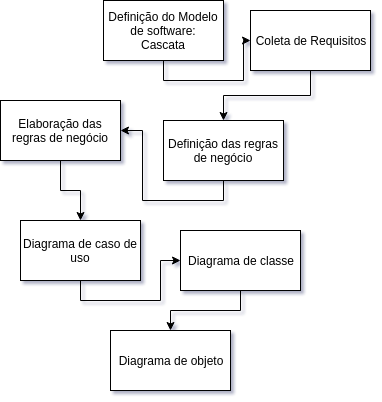
\includegraphics[width=\linewidth, frame]{Imagens/fluxograma.png}
        	\legend{Fonte: Elaboração própria}
        	\label{fig:flux}
        \end{figure}


    \subsection{Requisitos}
        Coletar requisito é uma parte fundamental do sistema, deve ser a fase inicial de qualquer software e assim pensar com clareza a melhor solução para as necessidades específicas do projeto, cada software possui suas características e prioridades, entendê-las é o papel da coleta de requisitos, e assim produzir um programa que atende as expectativas dos usuários.

        Os requisitos são uma abstração do que o sistema deve fazer, essas informações são coletadas através de sua engenharia, mesmo não sendo uma solução definitiva oferece uma base para um entendimento mais preciso, ajudando a compreender o problema, impacto do software, o que está sendo solicitado pelo cliente e como será a interação entre os usuários e o programa\cite[p.~116]{presman6ed}.
    
        Requisitos são divididos entre indispensáveis para o funcionamento do sistema e os que não estão ligados diretamente com o desempenho, mas sim com o comportamento, esses dois grupos são denominados de funcionais e não funcionais. \citeonline[p.~59]{ian_sommerville} mostra que os requisitos funcionais estão ligados aos serviços que o sistema oferece, da forma como ele deve-rá se comportar ao receber certos dados específicos ou até mesmo comportamentos que não devem ocorrer, já os não funcionais se trata de requisitos críticos para o programa, no qual especifica as restrições de serviços ou funções que em muitos casos se aplica ao software todo.


    \subsection{Regra de negócio}
        Gottesdiener \citeonline{gottesdiener1997business} afirma que as regras de negócios possuem diversos benefícios, como independência técnica, velocidade no desenvolvimento de aplicação, requisitos de melhor qualidade, ajuste facilitado e um equilíbrio entre flexibilidade e controle centralizado. São definidas como, “uma declaração que define ou restringe alguns aspectos do negócio” \cite[p.~4]{the_business_rules_group_guide_2000}. As restrições das regras de negócio são atômicas e não podem ser violadas, elas possuem o intuito de determinar como o negócio será organizado estruturalmente e de manter o controle ou induzir seu comportamento \cite[p.~5]{the_business_rules_group_guide_2000}.

        As regras de negócio podem ser vistas de duas perspectivas diferentes, da corporativa ou do sistema de informação, a perspectiva empresarial considera todos os comportamentos humanos na empresa como uma regra, desde restrições de proibido fumar a procedimentos para preencher um pedido. Já a perspectiva tecnológica se preocupa em restringir os dados que serão salvos e as mudanças que ocorrem, focando no que poderá ou não ser salvo no sistema \cite[p.~5]{the_business_rules_group_guide_2000}.
    
    
    \subsection{UML}
        A UML é essencial para melhorar a visualização da estrutura do sistema, facilitar o desenvolvimento e aumentar a compreensão e comunicação dos envolvidos na construção do software, é uma linguagem unificada de modelagem, que utiliza representações gráficas para visualizar, construir e documentar o desenvolvimento de um sistema. É padronizada, e oferece o que é necessário para projetar a arquitetura do programa, que vai dos aspectos conceituais aos concretos que estão ligados diretamente a sua construção \cite{booch_uml:_2006}.
    
    
    \subsection{Caso de uso}
        O caso de uso se trata de uma representação gráfica abstrata do funcionamento do sistema, é importante para auxiliar na coleta de requisitos através de um detalhamento das ações do usuário, é responsável por guia o processo de desenvolvimento \cite[p.~145]{videira_and_silva}.

        Os diagramas de caso de uso consistem em atores, cenários e relações, os atores representam o usuário ou função que irá realizar, ou sofrer uma ação, os cenários são uma série de ações que representa um comportamento do sistema, e as relações são a ligação entre um item e outro, especificando a interação entre os itens do diagrama.
        
        O objetivo principal do diagrama de caso de uso é representar o funcionamento do sistema de forma fácil de entender, focando nas funcionalidades que o programa deve desempenhar sem demonstrar como será feito \cite[p.~146]{videira_and_silva}.
        
    
    \subsection{Diagrama de classe}
        Diagramas de classes são um conjunto de vértices e arcos com nome e conteúdo, que representam classes, interfaces e colaborações com seus relacionamentos, sua principal função é realizar uma modelagem de uma visão estática do sistema, oferecendo suporte aos requisitos funcionais \cite[p.~109]{booch_uml:_2006}.

        Em uma abordagem orientada a objeto, o diagrama de classes se faz muito importante, para sistemas desenvolvidos com este conceito são um conjunto de classes e relacionamentos, ele oferece toda a organização e ligação que existirá no sistema, ao se pensar nessa estrutura com antecedência o processo de desenvolvimento torna-se e fácil, necessitando apenas transcrever o que está no diagrama para a linguagem de programação.
    
    
    \subsection{Diagrama de objeto}
        O diagrama de objeto está diretamente ligado ao de classes, ele representa a instância de uma classe, indicando o momento em que um conjunto de objetos relacionados executam uma ação, esta visão é uma representação estática do projeto ou do processo do sistema \cite[p.~188]{booch_uml:_2006}.

        Estas informações são úteis para entender as informações recebidos pelas classes ao executar certas operações, sendo relevante para a identificação de erros na entrada de dados das classes.
    
    
\section{Framework}
    Frameworks são ferramentas desenvolvidas com diversas funcionalidades pré-existentes para facilitar o desenvolvimento de software, é definido por \citeonline[p.~9]{opdyke1992refactoring} como um conjunto de classes abstratas e concretas, com o principal aspecto de ter sido pensado para ser sofisticado, permitindo o refinamento através de alterações ou criação de novos componentes.

    Uma ferramenta de qualidade deve oferecer funcionalidade de fácil entendimento e um ótimo funcionamento, o que não é diferente de ferramentas para desenvolvimento de software, de acordo com \citeonline[p.~9]{opdyke1992refactoring} os bons Frameworks possuem uma gama extensa de funções conectadas entre si, permitindo que os aplicativos possam se integrar por componentes existentes, e caso seja necessário criar um componente o mesmo será de simples, devido ao próprio framework produz um padrão e boa parte do código, além de exemplos.


\section{O Sistema WEB Cidadão do Vale}
    Conforme exposto à plataforma, Cidadão do Vale foi implementada no município de Almenara-MG como alternativa a informação de problemas urbanos e de gestão municipal. O sistema Cidadão do Vale foi disponibilizado de forma pública sob o domínio \url{http://u207457402.hostingerapp.com/}, em funcionamento completo que inclui a visualização e contribuição de dados do programa. Na Figura \ref{fig:cidInicio} é apresentada a página inicial, onde se encontra as colaborações georreferenciadas cadastradas no sistema em 3 de agosto de 2018. A Figura \ref{fig:cidCadastro} corresponde a tela de cadastro de usuário, e as Figuras \ref{fig:cidLimpeza} e \ref{fig:cidVias} correspondem aos mapas de calor referentes às contribuições sobre limpeza urbana e vias públicas em 3 de agosto de 2018.

    % PÁGINA INICIAL
    \begin{figure}[H]
    	\centering
    	\caption{Página inicial da plataforma Cidadão do Vale.}
    	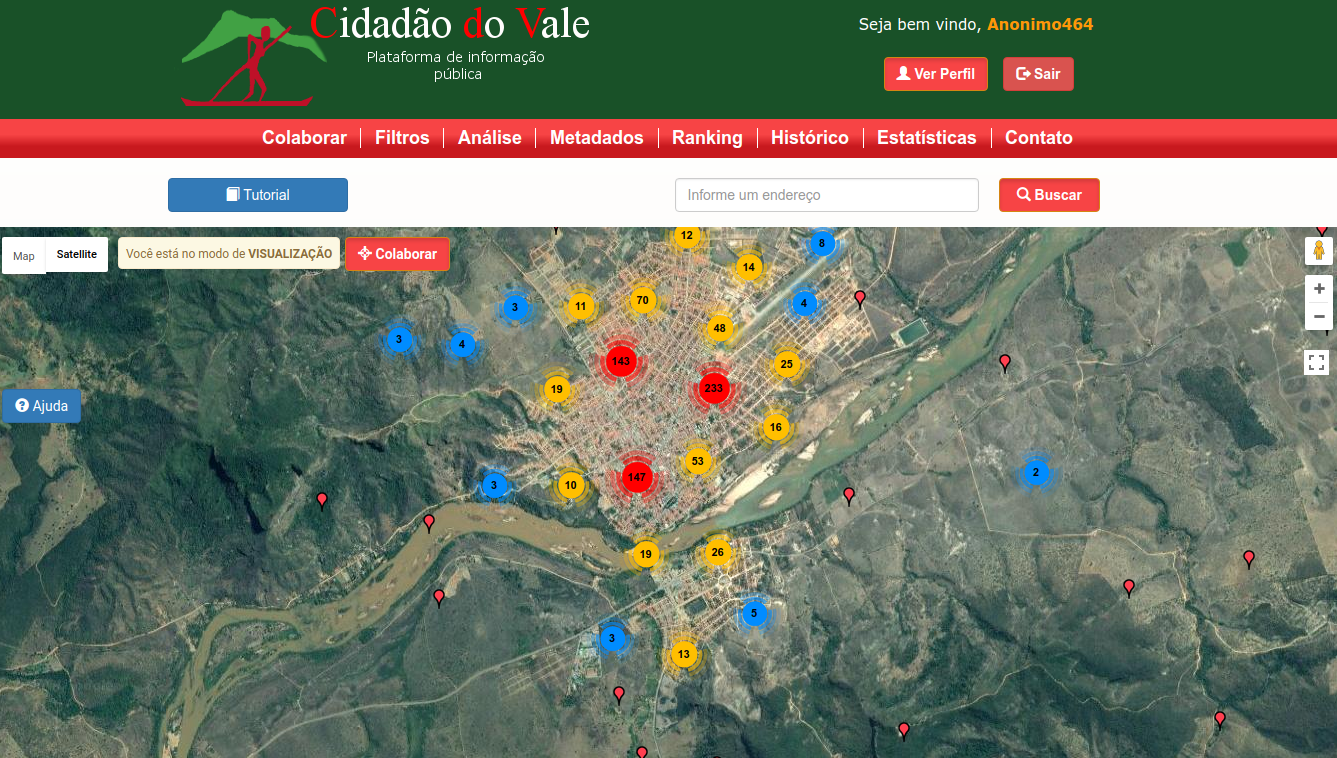
\includegraphics[width=0.6\linewidth]{Imagens/01}
    	\legend{Fonte: \url{http://u207457402.hostingerapp.com/}}
    	\label{fig:cidInicio}
    \end{figure}
    
    % CADASTRO
    \begin{figure}[H]
    	\centering
    	\caption{Página de cadastro do sistema Cidadão do Vale}	
    	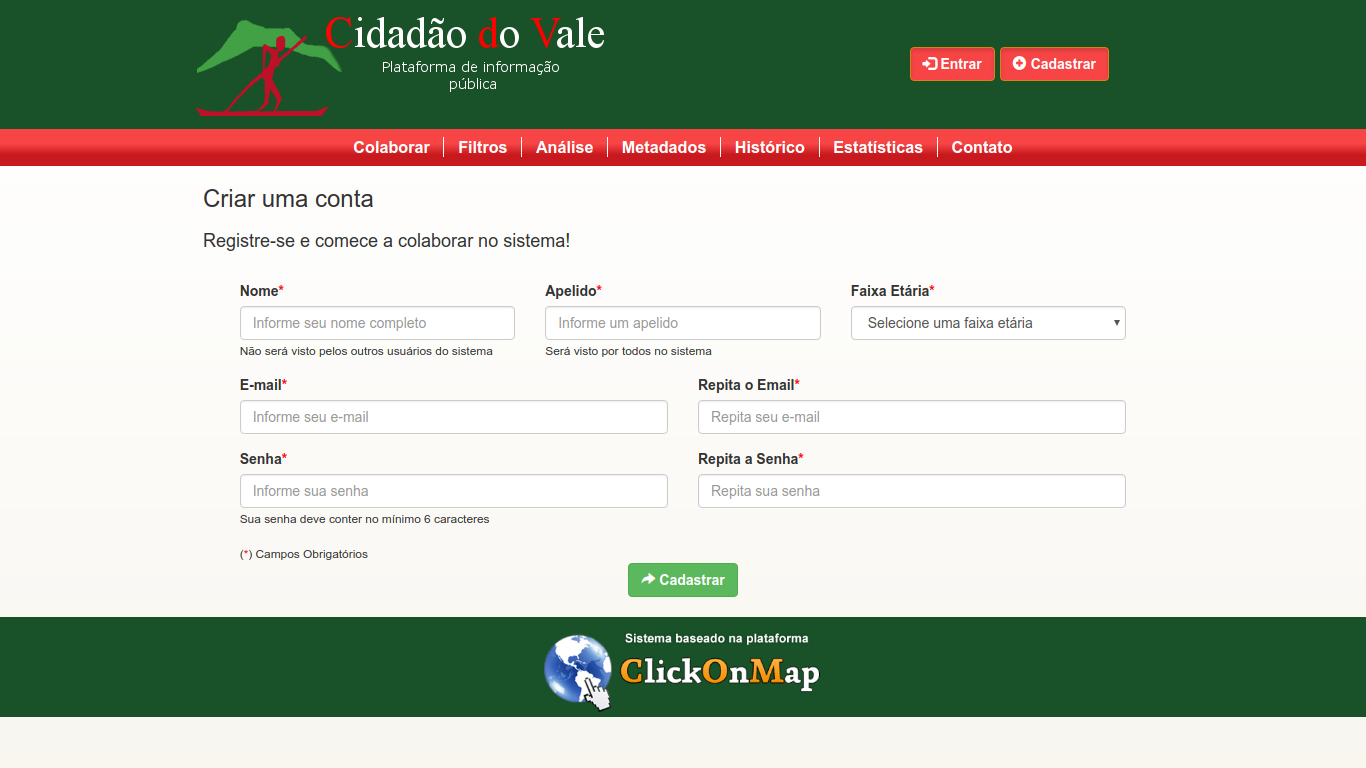
\includegraphics[width=0.6\linewidth]{Imagens/02}
    	\legend{Fonte: \url{http://u207457402.hostingerapp.com/registro.php}}
    	\label{fig:cidCadastro}
    \end{figure}
    
    % LIMPEZA URBANA
    \begin{figure}[H]
    	\centering
    	\caption{Densidade Kernel das contribuições sobre limpeza urbana.}
    	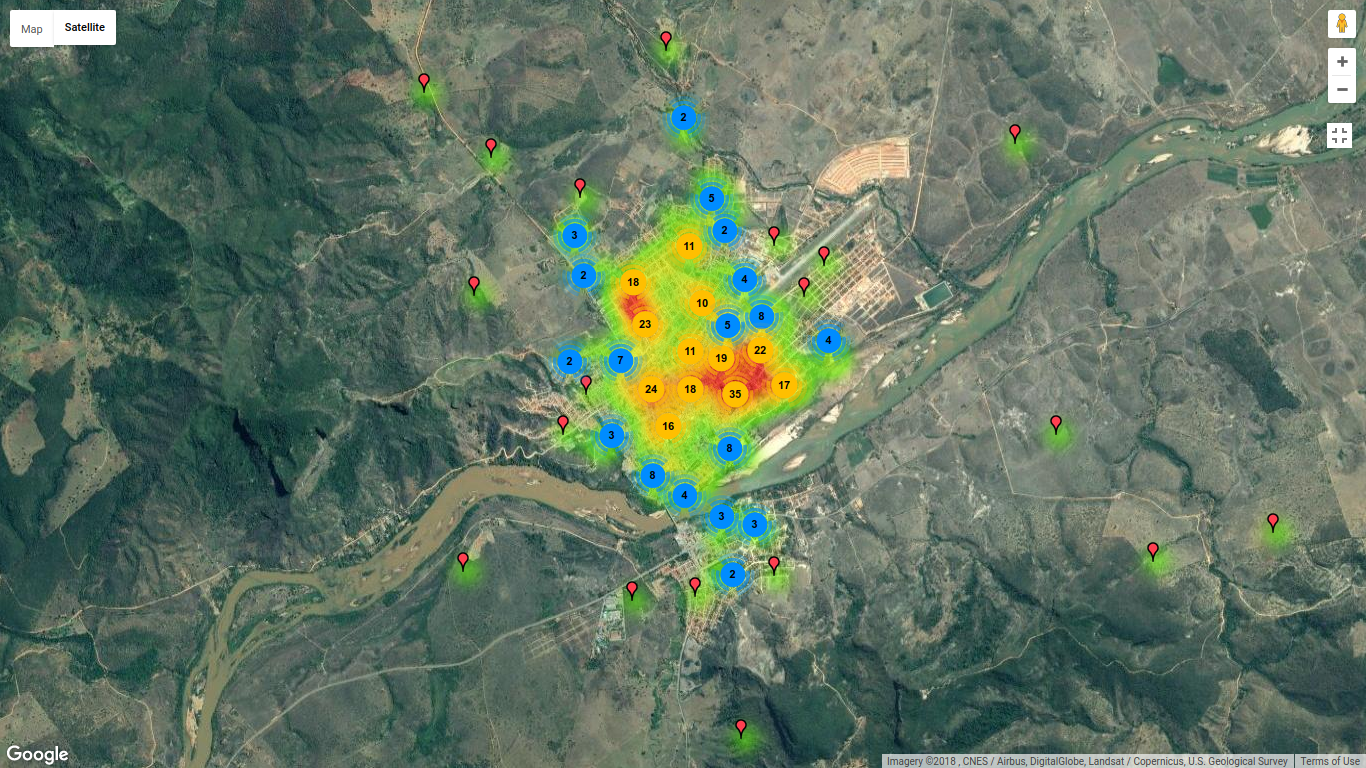
\includegraphics[width=0.6\linewidth]{Imagens/03}
    	\legend{Fonte: \url{http://u207457402.hostingerapp.com/}}
    	\label{fig:cidLimpeza}
    \end{figure}
    
    % VIAS PÚBLICAS
    \begin{figure}[H]
    	\centering
    	\caption{Densidade Kernel das contribuições sobre problemas nas vias públicas.}	
    	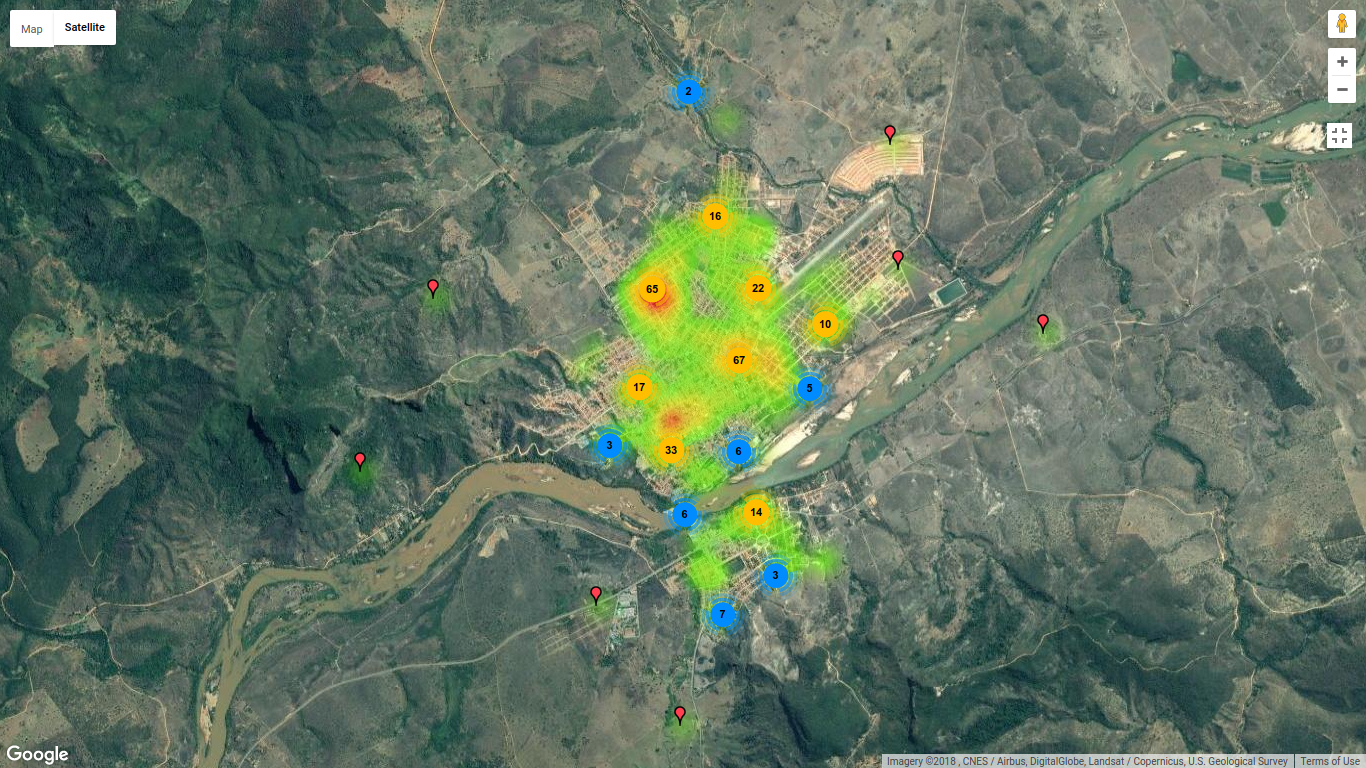
\includegraphics[width=0.6\linewidth]{Imagens/04}
    	\legend{Fonte :\url{http://u207457402.hostingerapp.com/}}
    	\label{fig:cidVias}
    \end{figure}

% esperar resposta e completar depois
\section{Sistemas semelhantes}
    Desenvolver um aplicativo para auxiliar na comunicação entre os cidadãos e a prefeitura da cidade não é uma novidade, atualmente já existem aplicativos que possuem esta finalidade. Apesar de serem aplicativos com os mesmos objetivos, são soluções que não permitem uma integração entre o aplicativo e a plataforma web, mas foram usados de base para projetar o sistema para a região.

    A pesquisa foi realizada na plataforma de aplicativos para Android, foram encontrados três sistemas brasileiros relevantes com maior quantidade de usuários, com a mesma temática do Cidadão do Vale. O primeiro é a plataforma Colab Figura \ref{fig:Colab}, é uma rede social para cidadania, que conecta o cidadão com a prefeitura das cidades. A plataforma Pelas Ruas Figura \ref{fig:pelasRuas}, permite que os usuários discutem e compartilham problemas da cidade de forma colaborativa. O aplicativo eCity Figura \ref{fig:eCity}, é uma plataforma colaborativa comum e simples, e seu estilo de tela limpa foi tomado como base para a criação dos protótipos.

    % Colab
    \begin{figure}[H]
    	\centering
    	\caption{Colab.}	
    	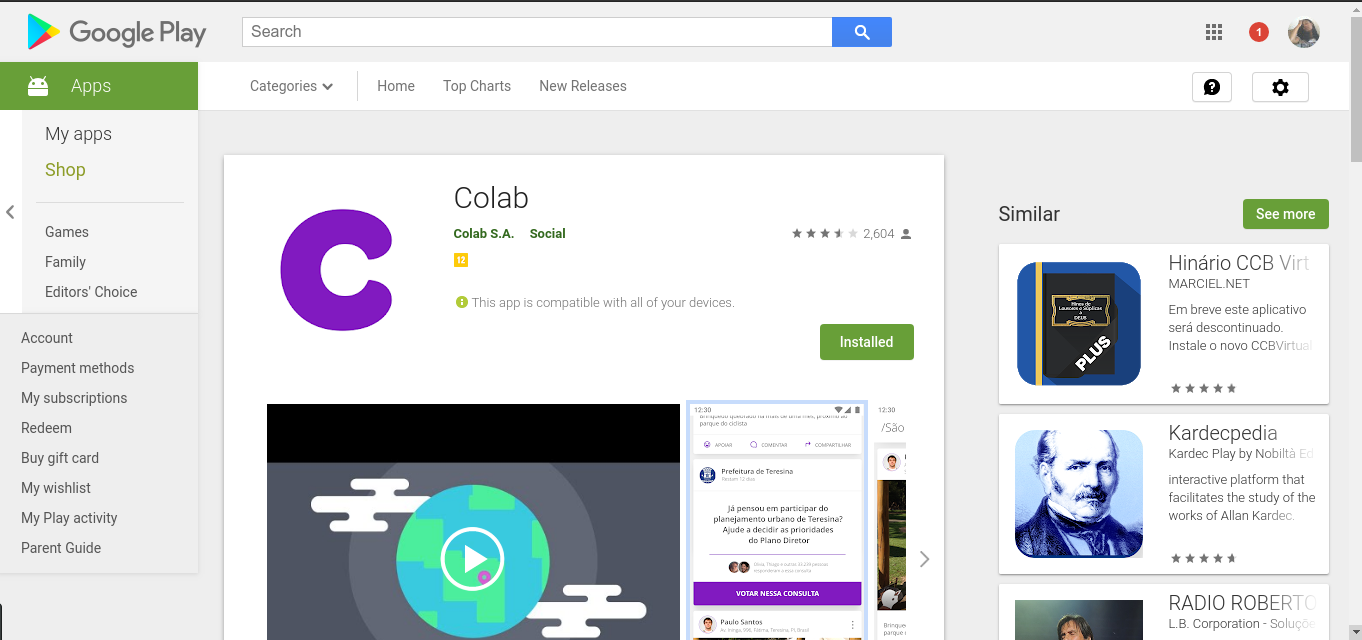
\includegraphics[width=\linewidth]{Imagens/app1.png}
    	\legend{Fonte: \url{https://play.google.com/store/apps/details?id=thirtyideas.colab_android}}
    	\label{fig:Colab}
    \end{figure}
    
    % Pelas Ruas
    \begin{figure}[H]
    	\centering
    	\caption{Pelas Ruas.}	
    	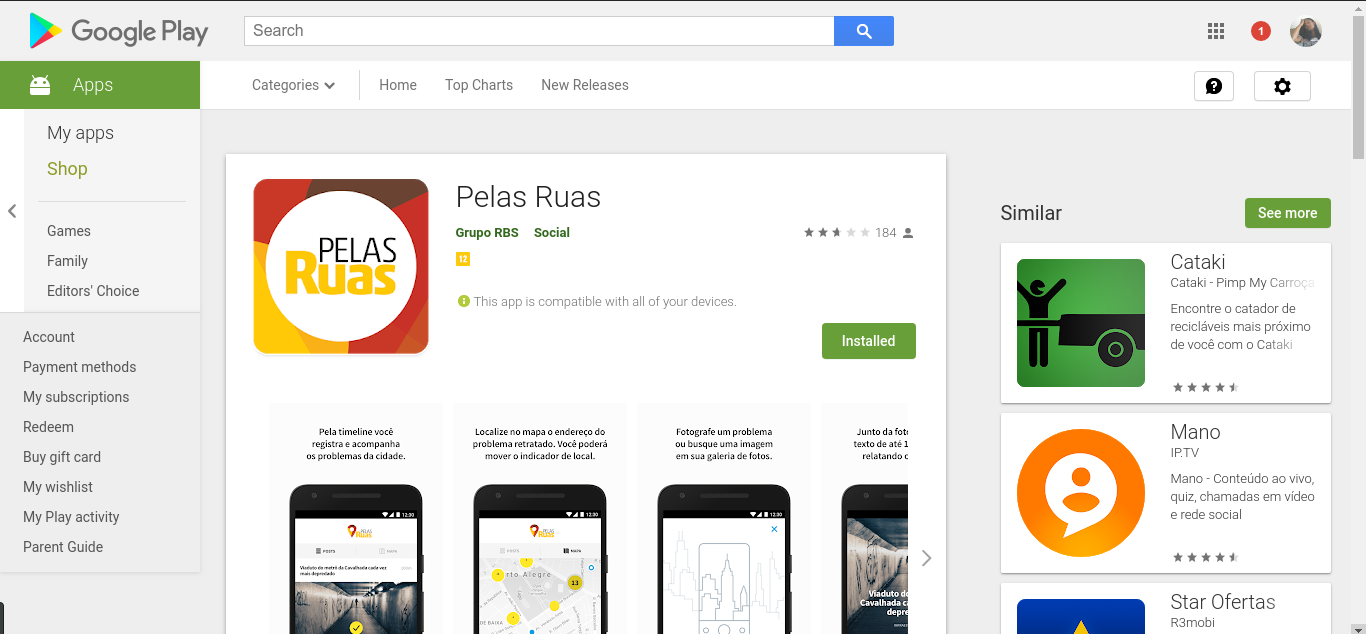
\includegraphics[width=\linewidth]{Imagens/app2.png}
    	\legend{Fonte: \url{https://play.google.com/store/apps/details?id=br.com.gruporbs.pelasruas}}
    	\label{fig:pelasRuas}
    \end{figure}
    
    % ECITY
    \begin{figure}[H]
    	\centering
    	\caption{ECITY.}	
    	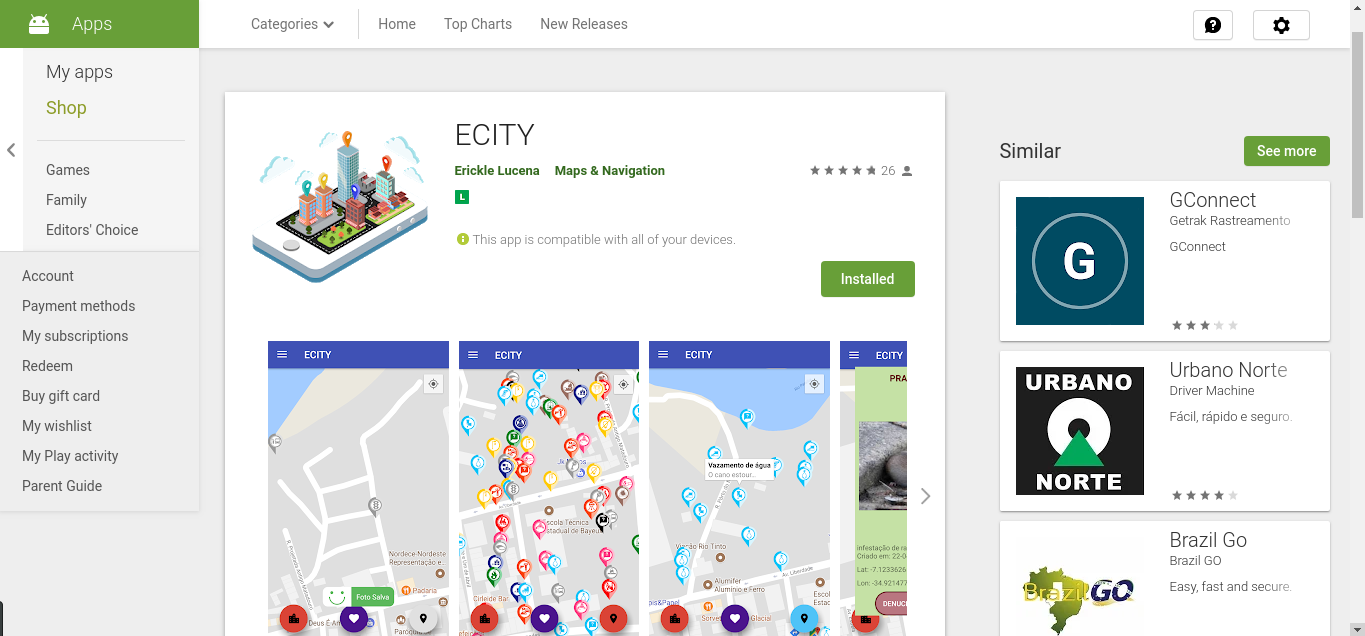
\includegraphics[width=\linewidth]{Imagens/app3.png}
    	\legend{Fonte: \url{https://play.google.com/store/apps/details?id=com.ecity.alice.project.ecity}}
    	\label{fig:eCity}
    \end{figure}
    
    
\section{Aplicativos nativos, Web Apps, ou híbridos?}    
    Foram avaliadas as características e vantagens de se desenvolver aplicativos dos tipos nativos, Web Apps, ou híbridos. Segundo informações de \citeonline{madureira_aplicativo_2017}, em síntese, eles se diferenciam pela linguagem utilizada e pelo tráfego de dados utilizados. Os nativos são programados em linguagem exclusiva para dispositivos móveis, são mais rápidos e confiáveis. Os Web Apps não são aplicativos reais, mas sim sistema web desenvolvidos para dispositivos móveis. As vantagens são o funcionamento em qualquer sistema operacional e o fato de não ocupar espaço na memória dos aparelhos. A desvantagem é que requer conexão com a internet para funcionamento. Por fim, os aplicativos híbridos são aqueles em que mesclam características dos nativos e Web Apps. Sua elaboração é mais simples, entretanto, requer internet para o funcionamento e não possui a mesma velocidade de resposta que um nativo.
    
\section{Cordova}
    Conforme apresentado na documentação oficial \citeonline{the_apache_software_foundation_architectural_nodate} o Cordova é um framework de código aberto que permite a utilização de linguagens da web para o desenvolvimento de aplicativos multiplataformas. Ele utiliza as linguagens padrão HTML5\footnote{Hypertext Markup Language — linguagem de marcação de hipertexto.}, CSS3\footnote{Cascading Style Sheets – estilo de folha em cascata.}, e JavaScript.

    \citeonline[p.~2]{lopes_sergio_aplicacao_2016} afirma que, o Cordova é responsável por criar uma “casca nativa” para o aplicativo, essa casca se trata de módulos menores que ficam dentro dos maiores, como uma casca e assim a comunicação é feita, por meio de uma janela de navegador, que se comunica entre as chamadas de código para nativas quando necessário. A Figura \ref{fig:codova} mostra a arquitetura do Cordova, na qual utiliza de APIs\footnote{Application programming interface.} para realizar a comunicação entre o sistema e a web, possibilitando assim o acesso a funcionalidades de qualquer aparelho, como sensores, dados, status da rede, etc.

    % Cordova arquitetura
    \begin{figure}[H]
    	\centering
    	\caption{Arquitetura do Cordova cria uma "casca nativa" para o aplicativo} 
    	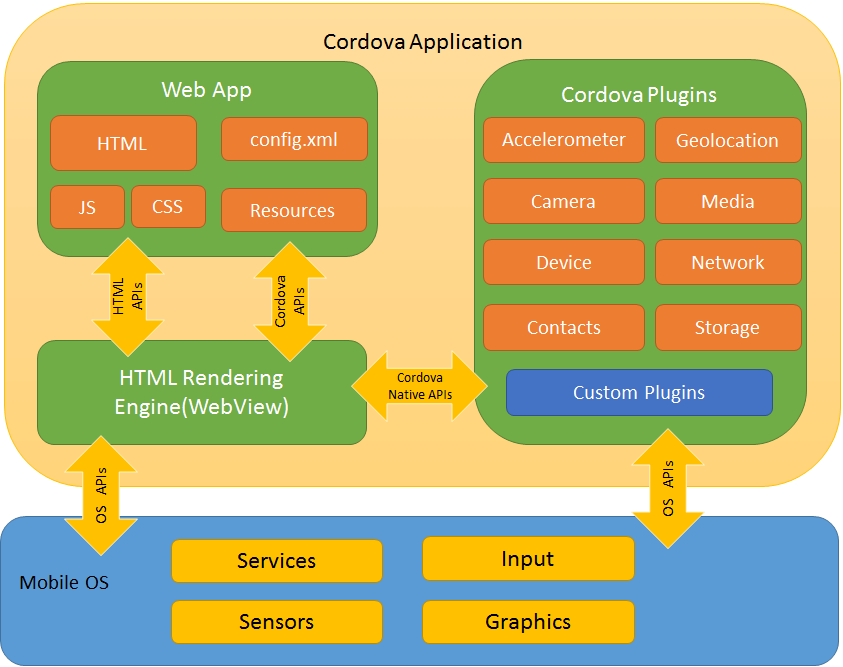
\includegraphics[width=0.6\linewidth]{Imagens/cordovaapparchitecture.png}
    	\legend{Fonte: \url{https://cordova.apache.org/docs/en/latest/guide/overview/index.html}}
    	\label{fig:codova}
    \end{figure}


\section{Firebase}
    O Firebase é um sistema online desenvolvido pela Google do qual possui vários serviços, como banco de dados em tempo real, acesso offline, \citeonline{khawas_application_2018} afirma que o Firebase é uma plataforma online, que auxilia os de desenvolvedores a criarem aplicações de qualidade, ele trabalha com armazenamento NoSQL, no qual realiza os armazenamentos em formato JSON\footnote{JavaScript Object Notation — Objeto de notação JavaScript}. Segundo \citeonline{silva_junior_and_buregio_vanilson_2016} o Firebase possui uma sincronização em tempo real para Android, iOS e JavaScript, que possibilita o aplicativo esteja responsivo e funcionando offline.

\section{NoSQL}
Os sistemas informatizados necessitam guardar dados, isso pode ser feito de diversas maneiras, em um arquivo, em um servidor ou em um banco de dados, a maneira mais comum é a utilização de banco de dados, podendo ser relacional ou não relacional, de acordo com \citeonline{vaish2013getting}, os banco de dados relacionais são muito utilizados até os dias de hoje,       são organizados em grupos com formato em tabelas linhas e colunas e por isso são considerados estruturados, pois os dados são muito bem definidos e organizados. O SQL é a linguagem comum para bancos de dados relacionais, que não é utilizada no NoSQL, pois não se trata de um banco relacional.

O conceito de NoSQL se trata de uma maneira não tradicional de organizar os dados, onde são tratados de forma não relacional, e não exigindo uma definição prévia dos tipos de dados que serão salvos, isso é feito de forma dinâmica, proporcionando maior liberdade de armazenamento e velocidade de acesso.